%%% -*-LaTeX-*-

\chapter{System Impact}
\label{chap:impact}

We saw how the Zero Copy promises savings of resources and enhanced performance 
in the previous chapters. To put things in the context of resource utilisation and
 to quantify performance gains, we profiled our benchmark code for memory bandwidth 
 and some other interesting metrics. One interesting observation from our initial 
 attempts was that our profiling code shouldn't interfere with the timing of our highly performant 
 benchmark which churns out millions of operations per second and microsecond latencies. 
 We searchaed for light weight profiling methods which adds minimal overheads.
 We ended up using Intel\textregistered's Performance Counter Monitoring module~\cite{intelpcm}. 
 An interesting thing about measuring performance 
 of a modern CPU is that almost all of the metrics of significance exist outside of the cores.
 The newer generation CPUs since the Sandy Bridge\textregistered microarchitecture provide an uncore performance 
 monitoring unit and we can use tools such as perf~\cite{perftool} to instrument these performance 
 counters. 

\section{Memory Bandwidth}
In a modern In-Memory Database server, DRAM utilisation is the most precious resource~\cite{ramcloudfast}. 
 Available memory bandwidth is also at a premium since there is a direct correlation between Memory Bandwidth
 utilisation and DRAM latencies and starvation. Since uncore events will give the most accurate measurements,
 we explored all uncore events that induce pressure on the memory controller. We found that 
\texttt{LLC\_MISSES X 64} (cache line size) is an interesting metric, but there was a problem that it wouldn't account for prefetch 
 misses. We went for the more accurate \texttt{MEMORY\_BW\_READS} and \texttt{MEMORY\_BW\_WRITES} metrics which are derived from 
 \texttt{CAS\_COUNT.RD} and \texttt{CAS\_COUNT.WR} metrics which are the number of cache lines read and written in the sampling 
 interval. We used an interactive reporting tool written on top of perf with named mappings for these events
 to measure this metric. We sampled total memory bandwidth consumed by the system while our benchmark 
 was running with fixed record sizes, number of records and mode of copying (Zero Copy and Copy Out).

\begin{figure}[t]
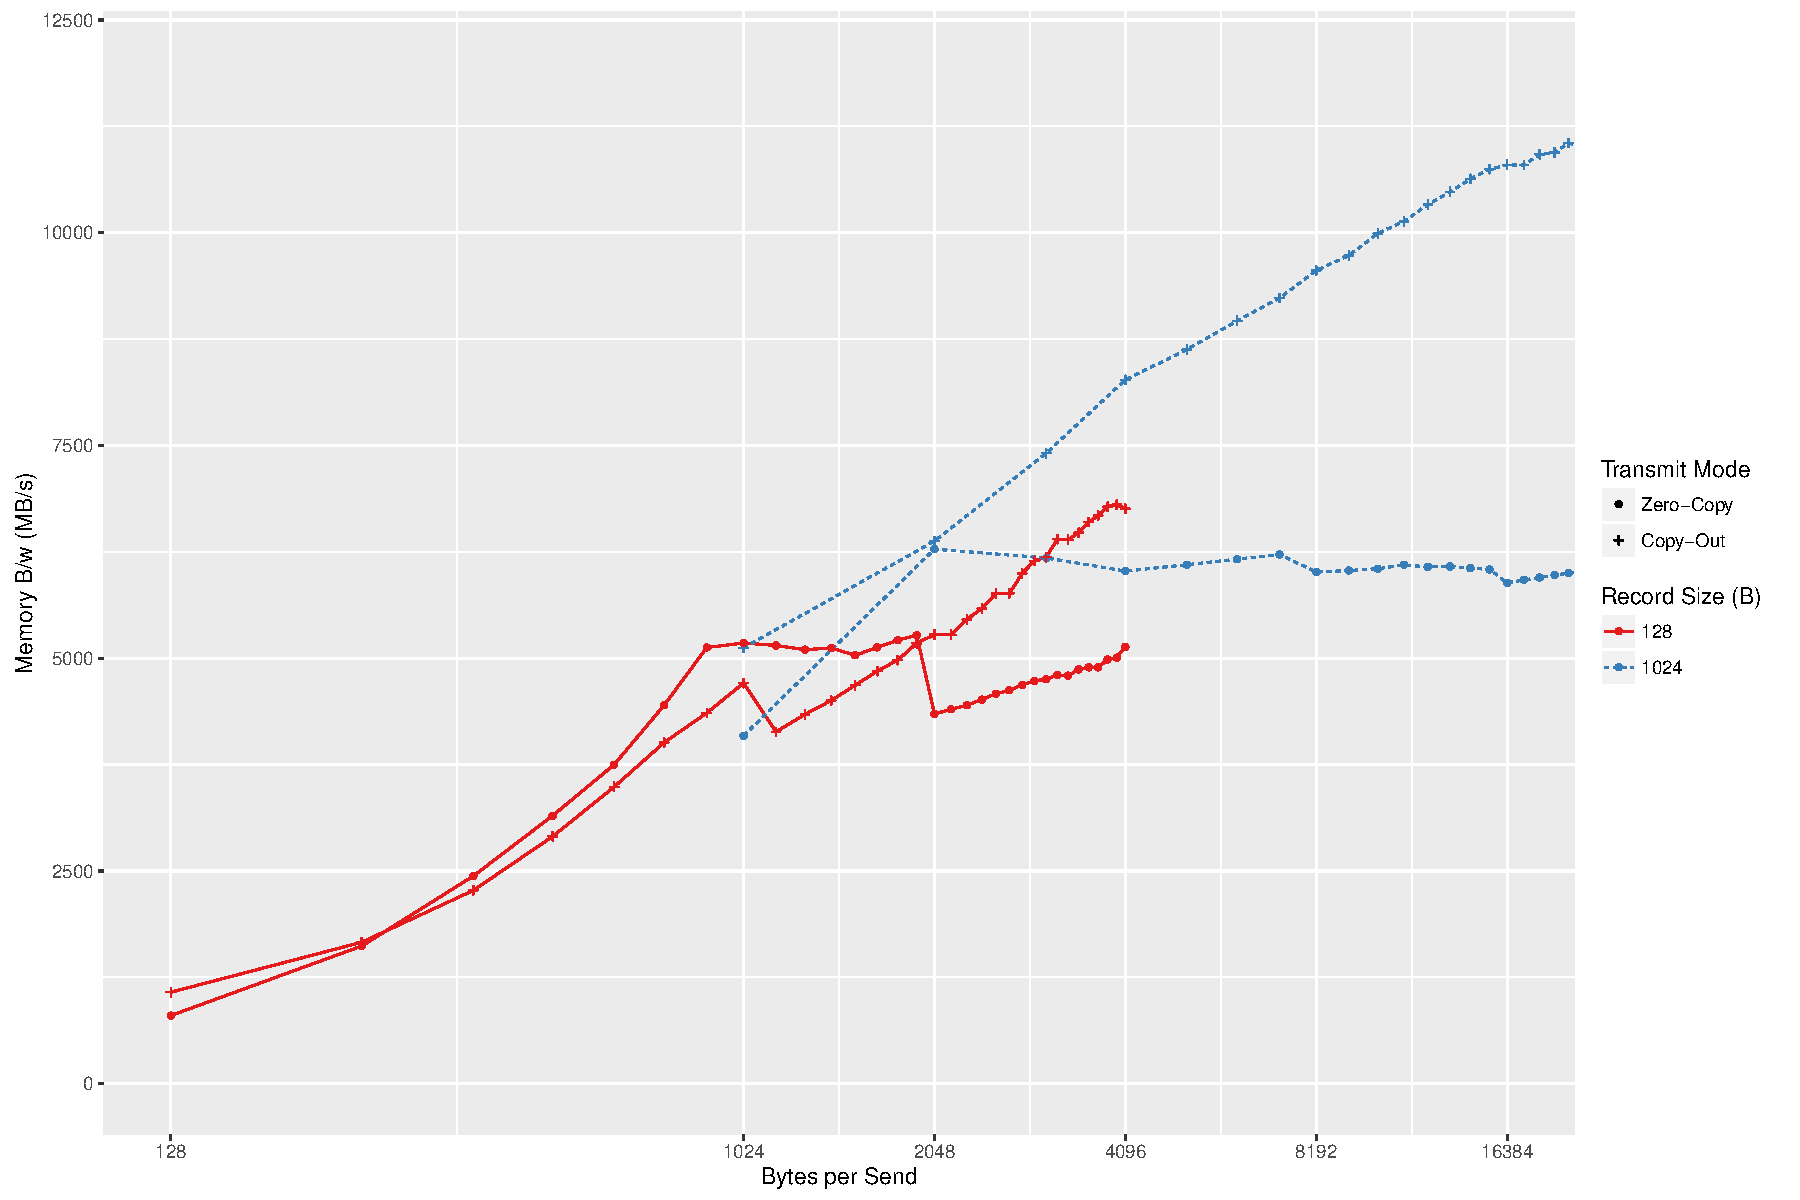
\includegraphics[width=\textwidth]{fig-membw.pdf}
\caption{Measured memory bandwidth impact on the system during transmission.}
\label{fig:membw}
\end{figure}


Figure ~\ref{fig:membw} shows the memory bandwidth consumed by the system while transmitting data at various modes 
of copying varying record sizes and transmission sizes. We can see that using zero copy on larger transmissions involving 
larger record sizes is clearly a win. The benefits are highlighted along largest transmissions of 32 records of sizes 1~KB each. 
 We had measured that a userspace application could achieve a peak bandwidth of 24~GB/s in our system. This would mean that Copy out 
 might hurt the system to the tune of a third of all available bandwidth. This is even more interesting considering that the modern day 
 In-memory stores are not tuned for large responses. When the DRAM latency and accesses go up, the performance of the whole system degrades.

For smaller data sizes, it's even more interesting. Zero Copy doesn't show a huge contrast in memory bandwidth utilisation. There are times 
when Copy out outperforms Zero Copy even in terms of memory bandwidth utilisations. Its interesting to note that these data points overlap the anomalous transmit performance 
degradation we saw while observing transmission throughput in Figure~\ref{fig:zero-copy-tput}. Interestingly, after this region in the graph 
where you transmit 16 or more 128~B records where Zero Copy offers better transmission throughput, the memory bandwidth consumption by Zero Copy 
is reduced and Copy-out starts to appear more expensive in terms of memory bandwidth. 

\subsection{Memory Bandwidth and Transmission throughput}
\begin{figure}[t]
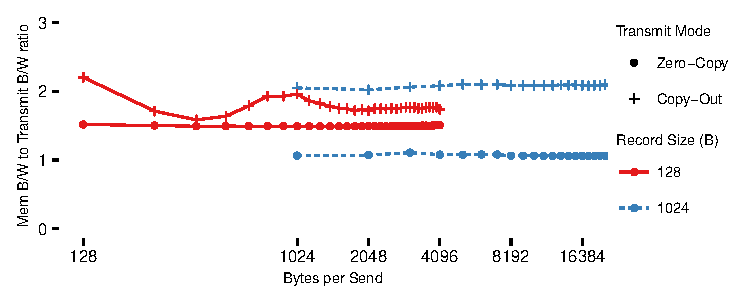
\includegraphics[width=\textwidth]{fig-membw-ratio.pdf}
\caption{Ratio of Memory Bandwidth to Transmission Throughput}
\label{fig:membw-ratio}
\end{figure}

Figure~\ref{fig:membw-ratio} shows the ratio of Memory pressure exerted per bytes transmitted. We can clearly see the value proposition of 
Zero Copy mode of transmitting here. For Zero Copy, We can see that the system is consistent and predictable and only incurs a tiny overhead of 
copying descriptors other than DMAing the data on to the NIC. The overhead of the descriptors is evident from the fact that 128~B records show 
a bigger multiplier on transmission throughput than 1024~B records. For 128~B records, the ratio appears tumultous across varying number of records, 
 but still shows Zero Copy as the clear winner. If we were to compare larger 1~KB records across the two modes of copying, we can see that there is a 
 2X memory bandwidth cost on copying out 1024~B records.

\section{DDIO traffic}
\begin{figure}[H]
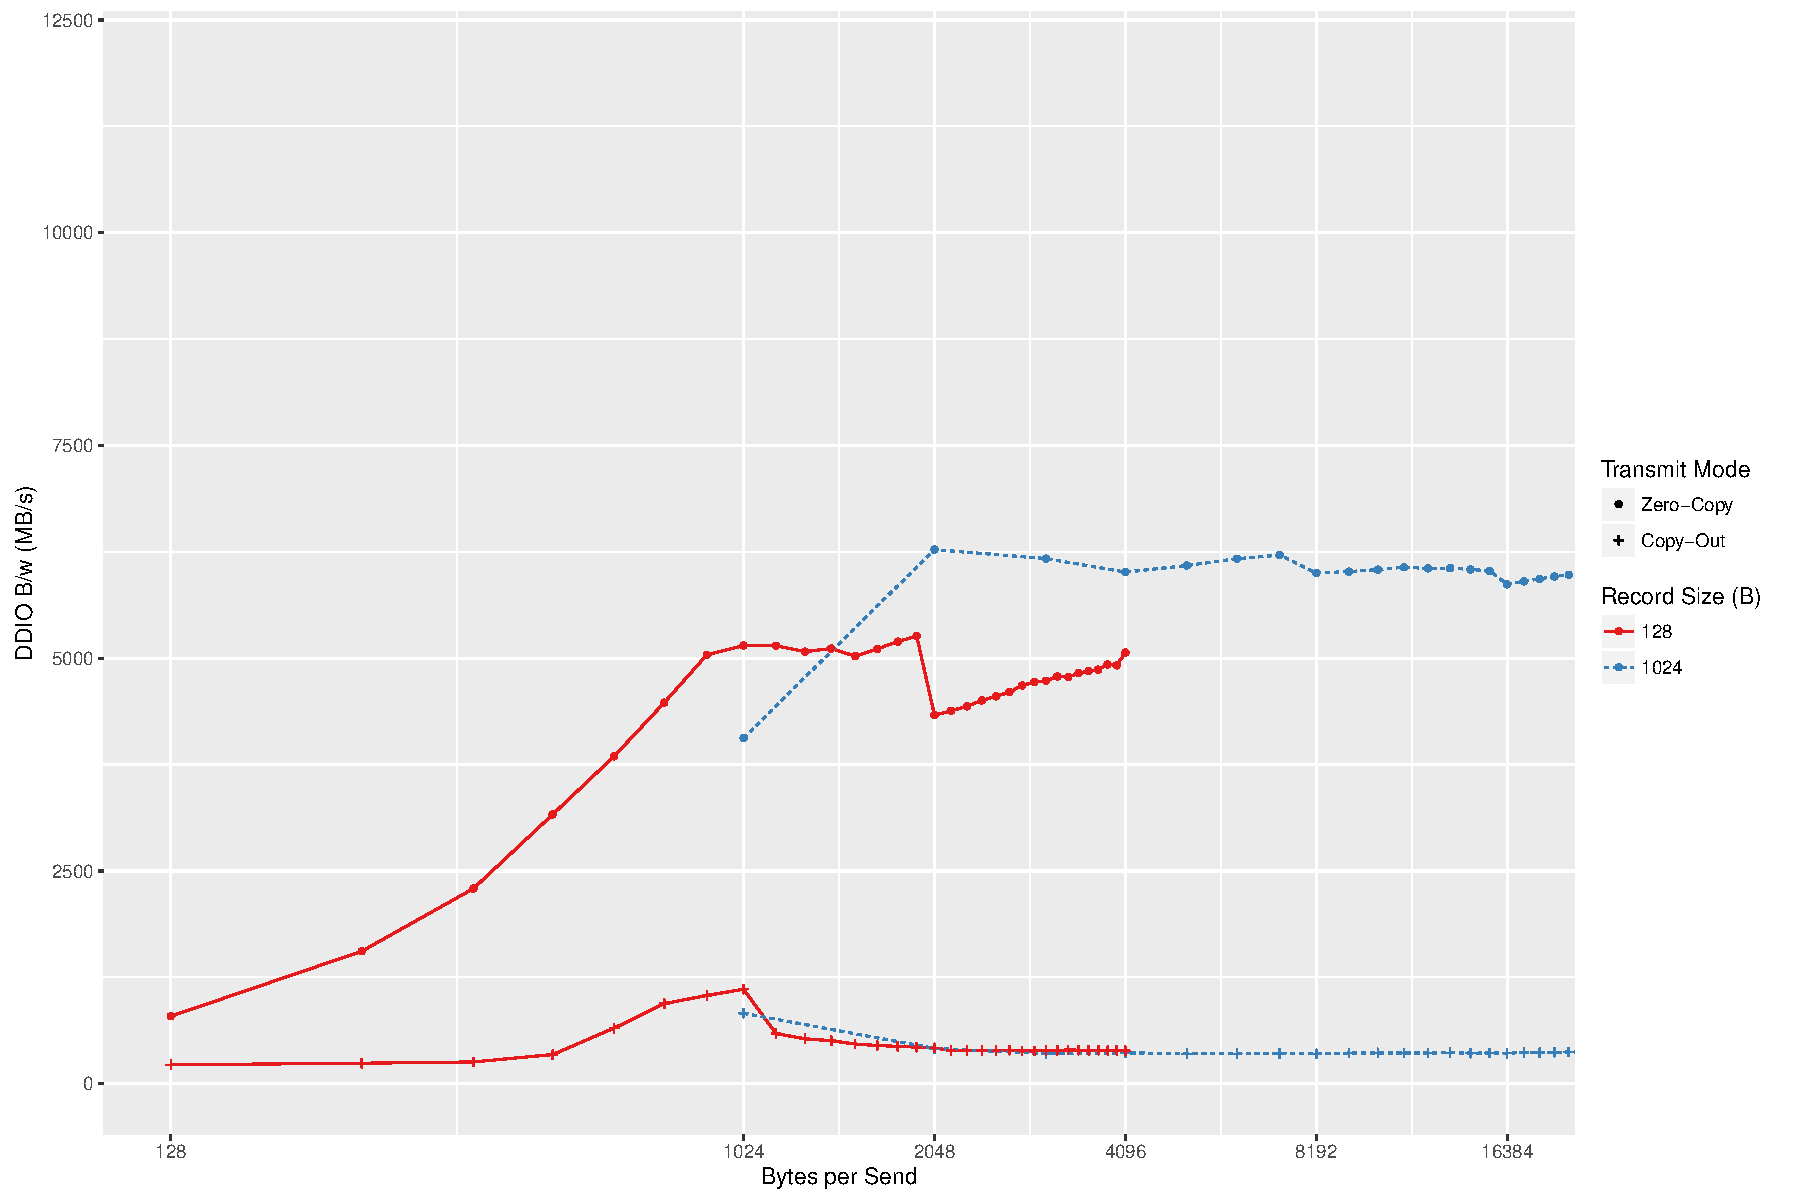
\includegraphics[width=\textwidth]{fig-ddiobw.pdf}
\caption{DRAM accesses (MB/s) LLC misses from DDIO vs Throughput}
\label{fig:ddiobw}
\end{figure}

Newer generation of Intel Processor's have a portion of their Last Level Cache dedicated for I/O. This was initially called Direct Cache Access\textregistered 
and more recently named DDIO\textregistered. This changes our perception of memory consumption quite a bit. Network transmission occurs at this part of the LLC 
and even the destination for a packet over the network becomes this dedicated portion of LLC. This has significant impact in the number of LLC misses the system 
has to take while dealing with network traffic. The key limitation to DDIO is that usually it's allocated as only 10\% of LLC which is around 2~MB in a modern system. 
But as long as a single transmission doesn't blow this size, we can expect higher efficiency in transmission. In all of our experiments, we were doing transmission of 
at most 32 records of 1~KB each and hence we can be sure that the effect of DDIO will be visible in our benchmarks. In order to measure the 
effect of DDIO, we measured the number of bytes read from memory by LLC due to misses from the DDIO region. 

Figure~\ref{fig:ddiobw} shows the reads issued to memory controller from LLC due to misses from the  DDIO region. We can clearly see that while we employ Copy out 
method to transmit data, we don't see much traffic in this area. When we issue a \memcpy~ to copy data into the transmit buffer, it's already loaded in the LLC. 
Unless that data is blown from LLC, a miss from the DDIO region need not necessarily involve a read from DRAM. On the other hand, if we were employing Zero Copy technique, 
and we were transmitting randomised chunks of data (We had to specifically turn this on to measure the effect), we can see that the DDIO misses follow the same trend 
as transmission throughput we showed in Figure~\ref{fig:zero-copy-tput}. Since our data sets are limited in size and doesn't cause much of cache pollution, we see that the 
memory reads due to misses in DDIO would not be as much as the total memory pressure inserted on the system. 

\section{Anomaly in Transmission Throughput}
While evaluating Zero Copy savings and performance in Chapter~\ref{chap:modernnics}, we saw that for 128~B records, the transmission throughput doesn't linearly progress 
while we increase the transmission size. While it trends upward until we reach 1024~B(8 records), the transmission throughput remains consistent for about 8-16 records and 
then the performance tapers off. There is a huge dip in transmission throughput going from 15 to 16 records and even though the performance gradually recovers, it doesn't quite 
catch up with Copy Out until we get to the maximum number of records possible and even at that point Copy Out edges Zero Copy performance by a bit. This was a bit puzzling 
for us in the beginning since Zero Copy showed promising transmit performance over almost all of the other scenarios. When we started measuring uncore event metrics, we noticed 
that LLC bytes read from memory due to misses from PCIe traffic, we found our answer to this.

\begin{figure}[t]
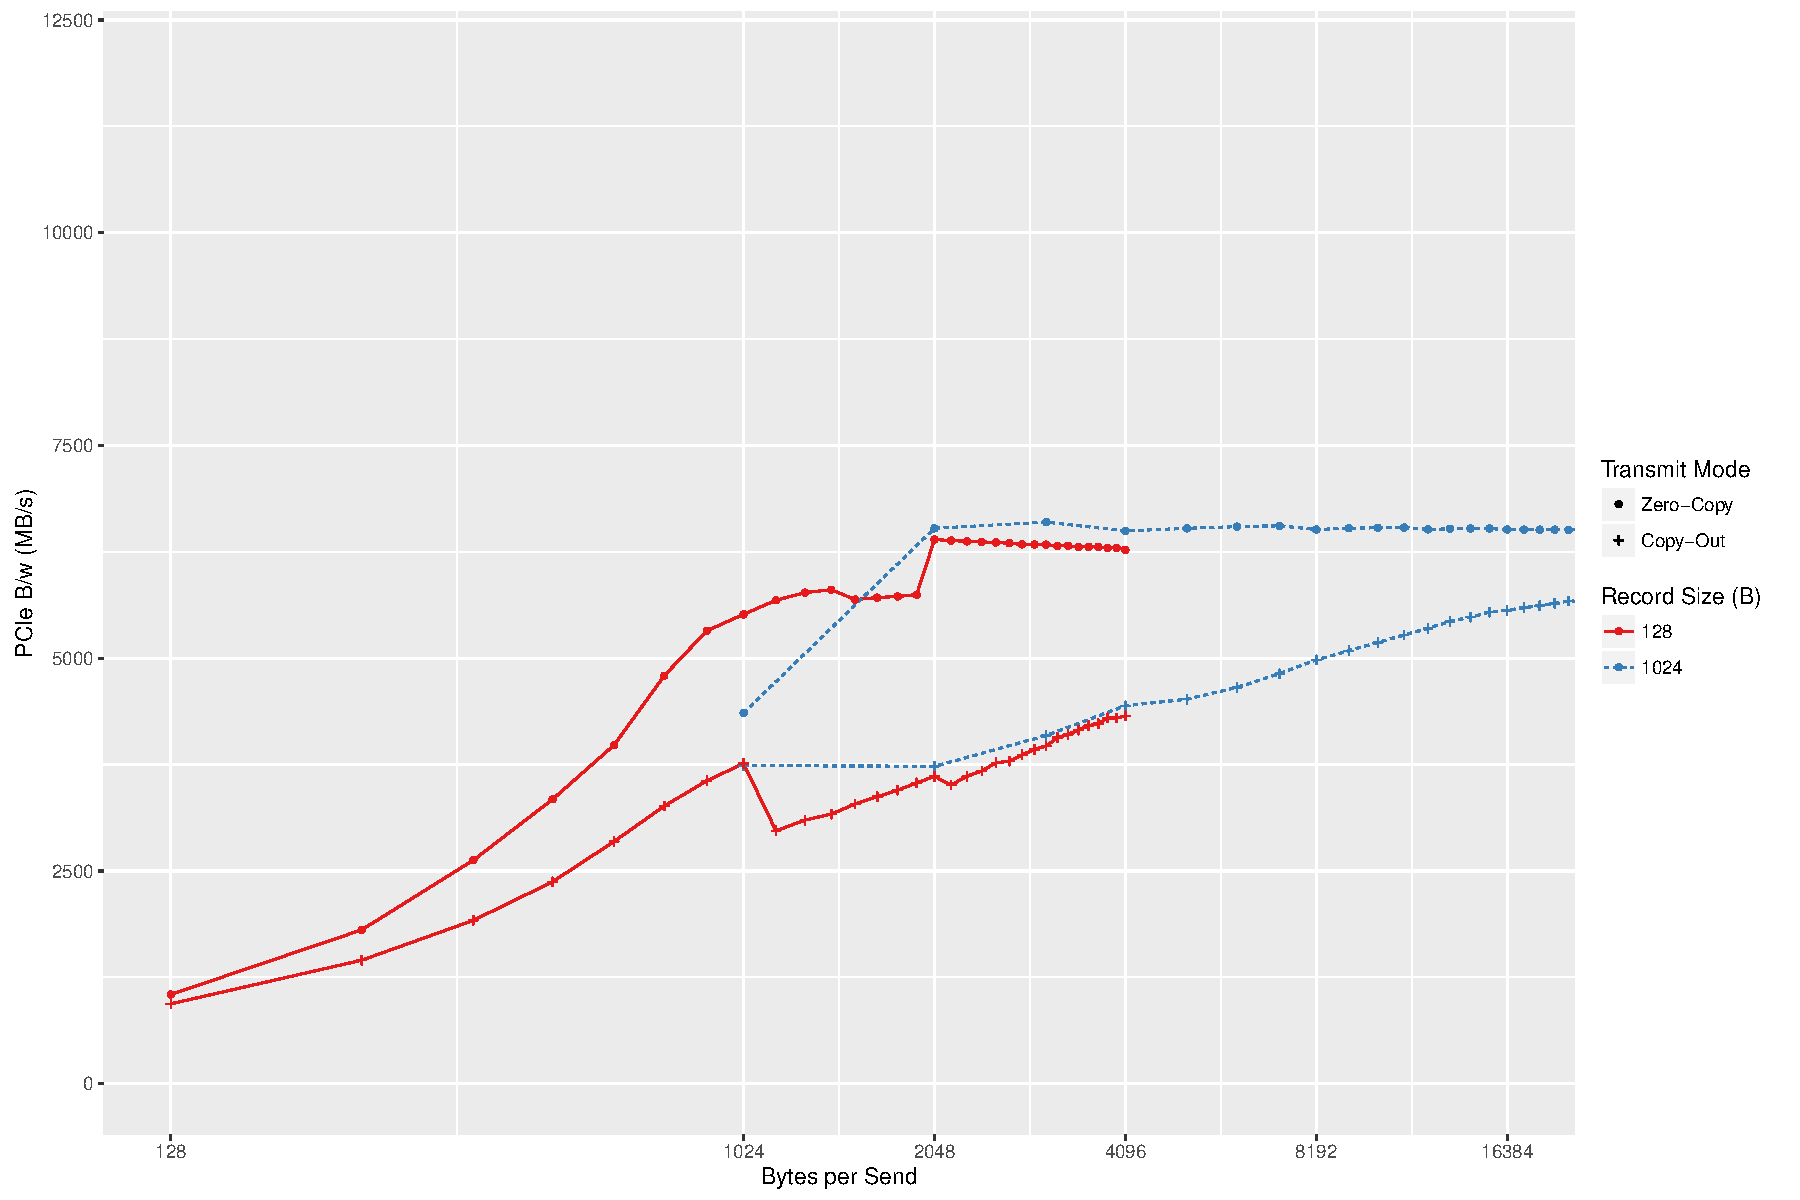
\includegraphics[width=\textwidth]{fig-pciebw.pdf}
\caption{DRAM accesses (MB/s) due to LLC misses due to PCIe}
\label{fig:pciebw}
\end{figure}


Figure~\ref{fig:pciebw} shows the read requests issued by LLC because of misses from PCIe traffic. For 128~B records, we can clearly see that after 8 records, this metric is 
nearly saturated and at 16 records, the number of bytes read peaks causing the dip in transmit performance. The memory reads due to PCIe traffic is saturated at this point and 
we can see a similar trend for 1024~B records too. Since larger records packs more data per record, the dip in transmit performance is not evident in that case. The other interesting 
thing to realise is that for Copy Out, the amount of memory traffic induced by PCIe follows a similar trend as transmission throughput which is expected since 
NIC itself is connected via PCIe interface.

